\documentclass{standalone}
\usepackage{tikz}
\begin{document}
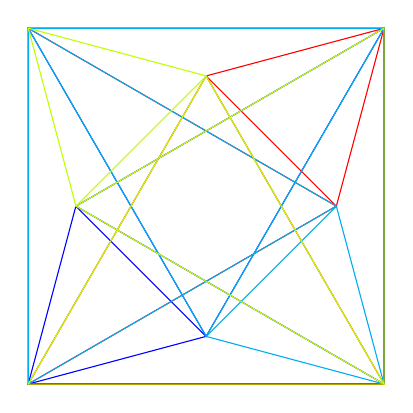
\begin{tikzpicture}[x=1pt,y=1pt]
\draw (208.88,-40.11) -- (80.32,-40.11) -- (80.32,-168.67) -- (208.88,-168.67) -- cycle;
\draw[red] (191.65,-104.39) -- (80.31,-168.67) -- (80.31,-40.11) -- cycle;
\draw[red] (191.65,-104.39) -- (144.60,-57.34) -- (208.88,-40.12) -- cycle;
\draw[red] (144.60,-57.34) -- (208.88,-168.67) -- (80.32,-168.67) -- cycle;
\draw[blue] (97.54,-104.39) -- (208.87,-40.11) -- (208.87,-168.67) -- cycle;
\draw[blue] (144.60,-151.45) -- (80.32,-40.12) -- (208.88,-40.12) -- cycle;
\draw[blue] (80.31,-168.68) -- (97.53,-104.40) -- (144.58,-151.45) -- cycle;
\draw[cyan] (144.60,-151.45) -- (80.32,-40.12) -- (208.88,-40.12) -- cycle;
\draw[cyan] (191.66,-104.39) -- (80.33,-168.67) -- (80.33,-40.11) -- cycle;
\draw[cyan] (208.88,-168.68) -- (144.60,-151.46) -- (191.65,-104.41) -- cycle;
\draw[lime] (208.88,-168.68) -- (80.32,-168.68) -- (144.60,-57.34) -- cycle;
\draw[lime] (144.60,-57.33) -- (97.55,-104.38) -- (80.33,-40.10) -- cycle;
\draw[lime] (97.54,-104.39) -- (208.87,-40.11) -- (208.87,-168.67) -- cycle;
\end{tikzpicture}
\end{document}
